\documentclass{beamer}
\usepackage[utf8]{inputenc}
\usepackage{graphicx} % Required for including images
\usepackage{tikz} % Required for diagrams
\usetikzlibrary{shapes, arrows, positioning, backgrounds, fit, calc} % For TikZ diagrams

\usetheme{Madrid} % A standard, clean theme
\usecolortheme{beaver} % More appealing color scheme
\setbeamertemplate{navigation symbols}{} % Remove navigation symbols
\setbeamertemplate{footline}[frame number]

\definecolor{rxblue}{RGB}{30,90,150}
\definecolor{rxgreen}{RGB}{60,179,113}
\definecolor{rxpurple}{RGB}{106,90,205}
\definecolor{rxorange}{RGB}{255,140,0}
\definecolor{rxwhite}{RGB}{245,245,245}

\title[RxPlain]{RxPlain: Simplifying Medical Information}
\author[Team]{Anubhav Shrestha \and Aymane Omari \and Bimarsha Adhikari \and Ronal Bista}
\institute[CS-UH 2012]{CS-UH 2012 Software Engineering}
\date{Spring 2025}

\begin{document}

% --- Title Page ---
\begin{frame}
  \titlepage
\end{frame}

% --- Table of Contents ---
\begin{frame}
  \frametitle{Presentation Outline}
  \tableofcontents
\end{frame}

% --- Introduction and Project Scope (1 min) ---
\section{Introduction \& Project Scope}
\begin{frame}
  \frametitle{Team Introduction \& Roles}
  
  \begin{itemize}
    \item \textbf{Anubhav Shrestha:} Frontend Development
    \item \textbf{Aymane Omari:} Backend Integration
    \item \textbf{Bimarsha Adhikari:} AI/LLM Integration
    \item \textbf{Ronal Bista:} Testing \& DevOps
  \end{itemize}
  
  \vspace{0.5cm}
  \begin{alertblock}{Project Overview}
    RxPlain empowers patients to understand their medical documents and medication interactions through AI-assisted simplification.
  \end{alertblock}
\end{frame}

\begin{frame}
  \frametitle{Project Objectives}
  
  \begin{itemize}
    \item \textbf{Simplify} complex medical terminology for patients
    \item \textbf{Identify} potential medication interactions
    \item \textbf{Generate} easy-to-follow medication schedules
    \item \textbf{Enable} healthcare provider verification of interpretations
    \item \textbf{Improve} patient understanding of health information
  \end{itemize}
  
  \vspace{0.5cm}
  \begin{center}
    \large{\textcolor{rxgreen}{Making medical information accessible to everyone}}
  \end{center}
\end{frame}

% --- Requirements (1 min) ---
\section{Requirements}
\begin{frame}
  \frametitle{Use Cases (1/2)}
  
  \begin{description}
    \item[\textcolor{rxgreen}{UC 1.1: Upload Medical Document}] \hfill \\
    Patient securely uploads a medical document (PDF, image) to the system
    
    \item[\textcolor{rxgreen}{UC 1.2: Simplify Document}] \hfill \\
    System uses LLM to transform complex medical terms into simple language
    
    \item[\textcolor{rxgreen}{UC 1.3: Check Medication Interactions}] \hfill \\
    System identifies and reports potential drug interactions with severity levels
  \end{description}
\end{frame}

\begin{frame}
  \frametitle{Use Cases (2/2)}
  
  \begin{description}
    \item[\textcolor{rxgreen}{UC 1.4: Verify Medical Document Interpretation}] \hfill \\
    Healthcare provider reviews and endorses or flags system interpretations
    
    \item[\textcolor{rxgreen}{UC 1.5: Generate Medication Schedule}] \hfill \\
    System generates an optimized medication schedule based on interaction analysis
  \end{description}
  
  \vspace{0.5cm}
  \begin{center}
    \textit{All use cases are fully implemented and will be demonstrated}
  \end{center}
\end{frame}

\begin{frame}
  \frametitle{Non-Functional Requirements (1/2)}
  
  \begin{block}{\textcolor{rxwhite}{Security}}
    \begin{itemize}
      \item Firebase Authentication
      \item Secure document storage
      \item Role-based access control
      \item Data encryption
    \end{itemize}
  \end{block}
  
  \begin{block}{\textcolor{rxwhite}{Performance}}
    \begin{itemize}
      \item API retry mechanisms
      \item Caching for faster responses
      \item Optimized document processing
    \end{itemize}
  \end{block}
\end{frame}

\begin{frame}
  \frametitle{Non-Functional Requirements (2/2)}
  
  \begin{block}{\textcolor{rxwhite}{Usability}}
    \begin{itemize}
      \item Responsive design
      \item Intuitive navigation
      \item Accessibility considerations
      \item Clear error messaging
    \end{itemize}
  \end{block}
  
  \begin{block}{\textcolor{rxwhite}{Reliability}}
    \begin{itemize}
      \item Error handling
      \item Quality verification
      \item Graceful degradation
      \item Comprehensive testing
    \end{itemize}
  \end{block}
\end{frame}

% --- Design (1 min) ---
\section{Design}
\begin{frame}
  \frametitle{System Architecture}
  
  \begin{center}
    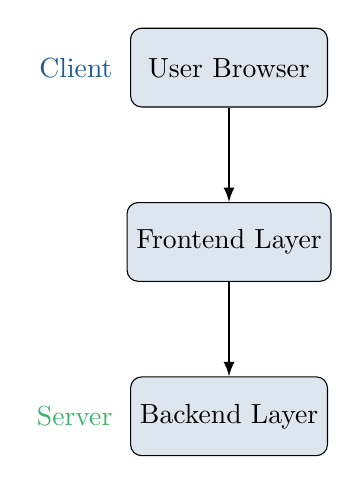
\begin{tikzpicture}[
      node distance=1.2cm,
      box/.style={rectangle, rounded corners, draw, fill=rxblue!15, 
        minimum width=2.5cm, minimum height=1cm, text centered},
      cloud/.style={ellipse, draw, fill=rxpurple!15, 
        minimum width=2.5cm, minimum height=1cm, text centered},
      arrow/.style={->, >=latex, thick},
      database/.style={cylinder, draw, shape aspect=0.3, fill=rxgreen!15,
        minimum height=1cm, minimum width=1.5cm, text centered}
    ]
      
      % Client Layer
      \node[box] (user) {User Browser};
      
      % Application Layer
      \node[box, below=of user] (frontend) {Frontend Layer};
      \node[box, below=of frontend] (backend) {Backend Layer};
      
      % Draw arrows
      \draw[arrow] (user) -- (frontend);
      \draw[arrow] (frontend) -- (backend);
      
      % Layer labels
      \node[left=0.1cm of user, text=rxblue] {Client};
      \node[left=0.1cm of backend, text=rxgreen] {Server};
    \end{tikzpicture}
  \end{center}
  
  \begin{center}
    \footnotesize{Simple 3-tier architecture with separation of concerns}
  \end{center}
\end{frame}

\begin{frame}
  \frametitle{System Architecture - External Services}
  
  \begin{center}
    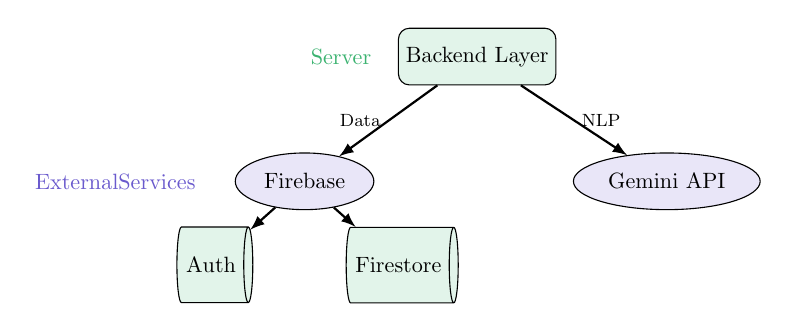
\begin{tikzpicture}[
      scale=0.8, transform shape,
      node distance=1.1cm,
      cloud/.style={ellipse, draw, fill=rxpurple!15, 
        minimum width=2.2cm, minimum height=0.9cm, text centered},
      arrow/.style={->, >=latex, thick},
      database/.style={cylinder, draw, shape aspect=0.3, fill=rxgreen!15,
        minimum height=0.8cm, minimum width=1.2cm, text centered}
    ]
      
      % Backend
      \node[rectangle, rounded corners, draw, fill=rxgreen!15, 
        minimum width=2.2cm, minimum height=0.9cm, text centered] (backend) {Backend Layer};
      
      % External Services - positioned closer to center
      \node[cloud, below left=1.2cm and 0.7cm of backend] (firebase) {Firebase};
      \node[cloud, below right=1.2cm and 0.7cm of backend] (gemini) {Gemini API};
      
      % Databases - positioned closer
      \node[database, below left=0.4cm and 0.1cm of firebase] (auth) {Auth};
      \node[database, below right=0.4cm and 0.1cm of firebase] (firestore) {Firestore};
      
      % Connections
      \draw[arrow] (backend) -- (firebase);
      \draw[arrow] (backend) -- (gemini);
      \draw[arrow] (firebase) -- (auth);
      \draw[arrow] (firebase) -- (firestore);
      
      % Labels for arrows
      \path (backend) -- (firebase) node[midway, left, font=\footnotesize] {Data};
      \path (backend) -- (gemini) node[midway, right, font=\footnotesize] {NLP};
      
      % Layer label
      \node[left=0.3cm of backend, text=rxgreen] {Server};
      \node[left=0.5cm of firebase, text=rxpurple] {External\\Services};
    \end{tikzpicture}
  \end{center}
  
  \begin{center}
    \footnotesize{Integration with Firebase for data/auth and Gemini API for AI functionalities}
  \end{center}
\end{frame}

\begin{frame}
  \frametitle{Class Diagram}
  
  \begin{center}
    \large{\textbf{Class Diagram Placeholder}}
    
    \vspace{1cm}
    \begin{itemize}
      \item Domain entities (Patient, HealthcareProvider, etc.)
      \item Service classes (LLM, System, StorageService)
      \item Key relationships (uploads, simplifies, verifies)
      \item GRASP patterns implementation
    \end{itemize}
  \end{center}
  
  \begin{center}
    \footnotesize{Final implemented class diagram showing key entities and relationships}
  \end{center}
\end{frame}

% --- Implementation and Testing (1 min) ---
\section{Implementation \& Testing}
\begin{frame}
  \frametitle{Tech Stack}
  
  \begin{columns}
    \begin{column}{0.5\textwidth}
      \begin{block}{\textcolor{rxwhite}{Frontend}}
        \begin{itemize}
          \item HTML5 / CSS
          \item Tailwind CSS
          \item Vanilla JavaScript
          \item Handlebars templates
        \end{itemize}
      \end{block}
      
      \begin{block}{\textcolor{rxwhite}{Backend}}
        \begin{itemize}
          \item Node.js
          \item Express.js
          \item RESTful API design
        \end{itemize}
      \end{block}
    \end{column}
    
    \begin{column}{0.5\textwidth}
      \begin{block}{\textcolor{rxwhite}{Database \& Auth}}
        \begin{itemize}
          \item Firebase Firestore
          \item Firebase Authentication
          \item Document-oriented storage
        \end{itemize}
      \end{block}
      
      \begin{block}{\textcolor{rxwhite}{AI \& Intelligence}}
        \begin{itemize}
          \item Google Gemini API
          \item Large Language Models
          \item Prompt engineering
        \end{itemize}
      \end{block}
    \end{column}
  \end{columns}
\end{frame}

\begin{frame}
  \frametitle{Challenges \& Solutions}
  
  \begin{itemize}
    \item \textbf{Challenge:} API Reliability \& Latency
    \item \textbf{Solution:} Implemented retry mechanism with exponential backoff
  \end{itemize}
  
  \vspace{0.4cm}
  
  \begin{itemize}
    \item \textbf{Challenge:} LLM Output Quality
    \item \textbf{Solution:} Added flagging system for uncertain simplifications
  \end{itemize}
  
  \vspace{0.4cm}
  
  \begin{itemize}
    \item \textbf{Challenge:} Test Coverage with ES Modules
    \item \textbf{Solution:} Used Node.js native testing for better compatibility
  \end{itemize}
\end{frame}

\begin{frame}
  \frametitle{Testing Results}
  
  \begin{block}{\textcolor{rxwhite}{Test Coverage}}
    \begin{center}
      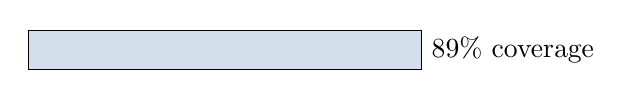
\begin{tikzpicture}
        \draw[fill=rxgreen!50] (0,0) rectangle (3,0.5);
        \draw[fill=rxorange!50] (3,0) rectangle (4,0.5);
        \draw[fill=rxblue!20] (0,0) rectangle (5,0.5);
        \node[right] at (5,0.25) {89\% coverage};
      \end{tikzpicture}
    \end{center}
  \end{block}
  
  \begin{block}{\textcolor{rxwhite}{Test Cases}}
    \begin{itemize}
      \item 25 test cases covering all 5 use cases
      \item Unit tests for critical components
      \item Integration tests for key workflows
      \item Mock components for external services
    \end{itemize}
  \end{block}
\end{frame}

% --- Demo (5 mins) ---
\section{Demo}
\begin{frame}
  \frametitle{Live Demonstration}
  
  \begin{center}
    \Huge\bfseries Demo Time!
  \end{center}
  
  \vspace{1cm}
  
  \begin{block}{\textcolor{rxwhite}{Features to Demo}}
    \begin{enumerate}
      \item Document Upload
      \item Document Simplification
      \item Medication Interaction Check
      \item Provider Verification
      \item Schedule Generation
    \end{enumerate}
  \end{block}
\end{frame}

\begin{frame}
  \frametitle{Demo Backup Plan}
  
  \begin{alertblock}{Video Demo Available}
    If needed, a recorded video demonstration is available
  \end{alertblock}
  
  \vspace{0.5cm}
  
  \begin{center}
    \Large\textbf{Video URL:}
    
    \url{https://youtu.be/2UBbypav6P8}
  \end{center}
  
  \vspace{0.5cm}
  
  \begin{center}
    \footnotesize{Video covers all five use cases with clear workflow examples}
  \end{center}
\end{frame}

% --- Conclusion ---
\section{Conclusion}
\begin{frame}
  \frametitle{From Requirements to Implementation: A Software Engineering Story}
  
  \begin{tikzpicture}[remember picture, overlay]
    \draw[rxheaderblue, line width=0.5pt] ([xshift=0cm, yshift=-0.9cm]current page.north west) -- ([xshift=\paperwidth, yshift=-0.9cm]current page.north west);
  \end{tikzpicture}
  
  \vspace{-0.3cm}
  
  \begin{bluebox}[The Power of Principled Design]
    \begin{itemize}
      \item[\textcolor{rxblue}{\faRobot}] \textbf{Information Expert} — AI services handled complex medical terminology translations
      \item[\textcolor{rxblue}{\faUserShield}] \textbf{Controller} — Authentication handlers kept user permissions separate from core app logic
      \item[\textcolor{rxblue}{\faLaptopCode}] \textbf{Low Coupling} — Document processing decoupled from interaction checking for modularity
      \item[\textcolor{rxblue}{\faChartBar}] \textbf{High Cohesion} — Each module handled one clear responsibility (simplification, scheduling, etc.)
      \item[\textcolor{rxblue}{\faUsers}] \textbf{Pure Fabrication} — Service classes coordinated complex multi-step user operations
    \end{itemize}
  \end{bluebox}
  
  \vspace{0.3cm}
  
  \begin{center}
    \begin{greenbox}
      \centering
      \textit{"GRASP patterns didn't just structure our code—they structured our thinking"}
    \end{greenbox}
  \end{center}
\end{frame}

\begin{frame}
  \frametitle{The Philosophy of Software Engineering}
  
  \begin{tikzpicture}[remember picture, overlay]
    \draw[rxheaderblue, line width=0.5pt] ([xshift=0cm, yshift=-0.9cm]current page.north west) -- ([xshift=\paperwidth, yshift=-0.9cm]current page.north west);
  \end{tikzpicture}
  
  \vspace{-0.3cm}
  
  \begin{bluebox}[Insights for a Future White Paper]
    \begin{itemize}
      \item[\textcolor{rxblue}{\faFileAlt}] Requirements are not specifications, but \textit{stories} that reveal human needs
      \item[\textcolor{rxblue}{\faCompass}] Design is a compass that guides implementation, not a constraint
      \item[\textcolor{rxblue}{\faTools}] GRASP patterns create a shared vocabulary for team problem-solving
      \item[\textcolor{rxblue}{\faBalanceScale}] The right balance between structure and flexibility produces maintainable code
      \item[\textcolor{rxblue}{\faHeartbeat}] Software isn't just lines of code—it's a living solution to human problems
    \end{itemize}
  \end{bluebox}
  
  \vspace{0.3cm}
  
  \begin{center}
    \begin{greenbox}
      \centering
      \large \textit{"Great engineers don't just build systems; they craft understanding."}
    \end{greenbox}
  \end{center}
  
  \vspace{0.3cm}
  
  \begin{center}
    \textcolor{rxgreen}{\large Thank You! Questions?}
  \end{center}
\end{frame}

\end{document}
